\documentclass[fleqn]{article}
\usepackage[nodisplayskipstretch]{setspace}
\usepackage{amsmath, nccmath, bm}
\usepackage{amssymb}
\usepackage{enumitem}
\usepackage{etoolbox}
\usepackage[normalem]{ulem}
\usepackage[hidelinks,colorlinks=true,urlcolor=blue,linkcolor=black]{hyperref}
\usepackage{graphicx}
\usepackage{float}
\usepackage{changepage}
\usepackage{environ,capt-of}
\usepackage{matlab-prettifier}

\let\oldfigure\figure% Store original figure float environment
\let\endoldfigure\endfigure
\RenewEnviron{figure}[1][H]{% Update figure environment
  %\par\vspace{\intextsep}% Assume in-text placement, so insert appropriate vertical spacing
  \noindent
  % \patchcmd{<cmd>}{<search>}{<replace>}{<success>}{<failure>}
  \patchcmd{\BODY}{\caption}{\captionof{figure}}{}{}% Replace \caption with \captionof{figure} inside \BODY
  % Set "figure"
  \begin{minipage}{\linewidth}
    \BODY
  \end{minipage}
  %\par\vspace{\intextsep}% Assume in-text placement, so insert appropriate vertical spacing
}

\makeatletter
\begingroup
  \catcode`\$=6 %
  \catcode`\#=12 %
  \gdef\href@split$1#$2#$3\\$4{%
    \hyper@@link{$1}{$2}{\uline{$4}}% or \underline
    \endgroup
  }%
\endgroup

\newcommand{\zerodisplayskip}{
	\setlength{\abovedisplayskip}{0pt}%
	\setlength{\belowdisplayskip}{0pt}%
	\setlength{\abovedisplayshortskip}{0pt}%
	\setlength{\belowdisplayshortskip}{0pt}%
	\setlength{\mathindent}{0pt}}
	
\title{Homework 5}
\author{Owen Sowatzke}
\date{April 12, 2024}

\begin{document}

	\offinterlineskip
	\setlength{\lineskip}{12pt}
	\zerodisplayskip
	\maketitle
	
	\begin{enumerate}
		\item Consider two 1D sequences $x(n)$ with 10 elements and $h(n)$ with 3 elements. Further, the sequence $x(n)$ can also be denoted by the vector $\mathbf{x}$ of length 10. Find a matrix $\mathbf{H}$ such that the product $\mathbf{y} = \mathbf{Hx}$ is identical to the correlation between $x(n)$ and $h(n)$, i.e. $y(n) = \sum_{k=1}^{10}{h(k+n-1)x(k)}$.
		
		\begin{enumerate}
			\item [1)] What are the dimensions of $\mathbf{H}$ assuming that we are interested in values $y(n)$ for which all samples of $h(n)$ are overlapping with samples of $x(n)$?
			
			The full convolution output is $N + M - 1$ samples long, where $N$ is the length of $x(n)$ and $M$ is the length of $h(n)$. At the start and tail of the convolution output, there are $M - 1$ samples during which all samples $h(n)$ are not overlapping with samples of $x(n)$. As such, the length of the valid convolution output is:
			
			$N + M - 1 - 2(M - 1) = N + M - 1 - 2M + 2 = N - M + 1$
			
			$ = 10 - 3 + 1 = 8$ samples .
			
			Therefore, the matrix $\mathbf{H}$ must transform the $10 \times 1$ input vector $\mathbf{x}$ into an $8 \times 1$ output vector $\mathbf{y}$.  As such $\mathbf{H}$ must be an $8 \times 10$ matrix.
			
			\item [2)] What is the size of the output vector $\mathbf{y}$?
			
			As stated above, $\mathbf{y}$ must be an $8 \times 1$ vector.
			
			\item [3)] What are the dimensions of $\mathbf{H}$ for the 2D case where $x(m,n)$ is a $10 \times 10$ image, and $h(m,n)$ is a $3 \times 3$ kernel, and the output is given by $y(m,n) = \sum{\sum{h(j+m-1,k+n-1)x(j,k)}}$? Assume that we are only considering values of $y(m,n)$ obtained when $h(m,n)$ is fully overlapped with $x(m,n)$. What is the size of $\mathbf{y}$ in this case?
			
			For the 2D case, each dimension of the output $y(n,m)$ will be $N - M + 1 = 8$ samples long. Therefore, the output $y(n,m)$ will be an $8 \times 8$ image. To perform 2D convolution using a matrix vector equation, $x(n,m)$ and $y(n,m)$ must be flattened to form vectors $\mathbf{x}$ and $\mathbf{y}$. After flattening, $\mathbf{x}$ will be $100 \times 1$ and $\mathbf{y}$ will be $64 \times 1$. Thus, the matrix $\mathbf{H}$ must be $64 \times 100$.
			
			\item[4)] What can you say about the structure of the matrix $\mathbf{H}$?
			
			For the 1D case, the matrix $\mathbf{H}$ can be written as follows:
			
			\begin{equation*}
				\mathbf{H} = \begin{bmatrix}
					h(3)   & h(2)   & h(1)   & 0      & \cdots & 0      & 0      & 0 \\
					0      & h(3)   & h(2)   & h(1)   & \cdots & 0      & 0      & 0 \\
					\vdots & \vdots & \vdots & \vdots & \ddots & \vdots & \vdots & \vdots \\
					0      & 0      & 0      & 0      & \cdots & h(2)   & h(1)   & 0 \\
					0      & 0      & 0      & 0      & \cdots & h(3)   & h(2)   & h(1)
				\end{bmatrix}
			\end{equation*}
				
			Therefore, for the 1D case, $\mathbf{H}$ is a Toeplitz matrix.
			
			For the 2D case, the matrix $\mathbf{H}$ can be written as follows:
			
			\begin{equation*}
				\mathbf{H} = \begin{bmatrix}
					\mathbf{H_1} & \mathbf{H_2} & \mathbf{H_3} & \mathbf{0}   & \cdots & \mathbf{0}   & \mathbf{0}   & \mathbf{0}   & \mathbf{0} \\
					\mathbf{0}   & \mathbf{H_1} & \mathbf{H_2} & \mathbf{H_3} & \cdots & \mathbf{0}   & \mathbf{0}   & \mathbf{0}   & \mathbf{0} \\
					\vdots       & \vdots       & \vdots       & \vdots       & \ddots & \vdots       & \vdots       & \vdots       & \vdots     \\
					\mathbf{0}   & \mathbf{0}   & \mathbf{0}   & \mathbf{0}   & \cdots & \mathbf{H_1} & \mathbf{H_2} & \mathbf{H_3} & \mathbf{0} \\
					\mathbf{0}   & \mathbf{0}   & \mathbf{0}   & \mathbf{0}   & \cdots & \mathbf{0}   & \mathbf{H_1} & \mathbf{H_2} & \mathbf{H_3} \\
				\end{bmatrix}
			\end{equation*}
			
			where $\mathbf{H_i}$ is given as follows:
			
			\begin{equation*}
				\mathbf{H_i} = \begin{bmatrix}
					h(3,i) & h(2,i) & h(1,i) & 0      & \cdots & 0      & 0      & 0 \\
					0      & h(3,i) & h(2,i) & h(1,i) & \cdots & 0      & 0      & 0 \\
					\vdots & \vdots & \vdots & \vdots & \ddots & \vdots & \vdots & \vdots \\
					0      & 0      & 0      & 0      & \cdots & h(2,i) & h(1,i) & 0 \\
					0      & 0      & 0      & 0      & \cdots & h(3,i) & h(2,i) & h(1,i)
				\end{bmatrix}
			\end{equation*}
			
			Therefore, for the 2D case, $\mathbf{H}$ is a block Toeplitz matrix.
		\end{enumerate}
		
		\item For this problem we will use the MNIST data:
		
		\href{https://git-disl.github.io/GTDLBench/datasets/mnist\_datasets/}{https://git-disl.github.io/GTDLBench/datasets/mnist\_datasets/}
		
		\begin{itemize}
			\item Modify the simple CNN discussed in class (see matlab script \newline simpleCNN\_cifar10.m) to work with the MNIST data by adjusting the parameters of the input layer. Train this network to obtain a 10-class classifier. You do not have to use matlab for your experiments, but the structure and number of parameters of the network should be the same as that in the matlab script.
			
			\item Evaluate the performance of the network on the test images and report the overall accuracy as well as the confusion matrix.
			
			\item Compare the performance of this network to a KNN classifier (K=3) in terms of overall accuracy and the confusion matrix. Which approach is better?
			
			\item Submit your code for training and testing the CNN.
			
		\end{itemize}
		
		Note: You can use any programming language and libraries for this \newline problem.
		
		\pagebreak
		
		When evaluated on the test data set, the CNN classifier achieved 99.04\% accuracy. The CNN classification results are displayed in the following confusion matrix:
		
		\begin{figure}[H]
			\centerline{\fbox{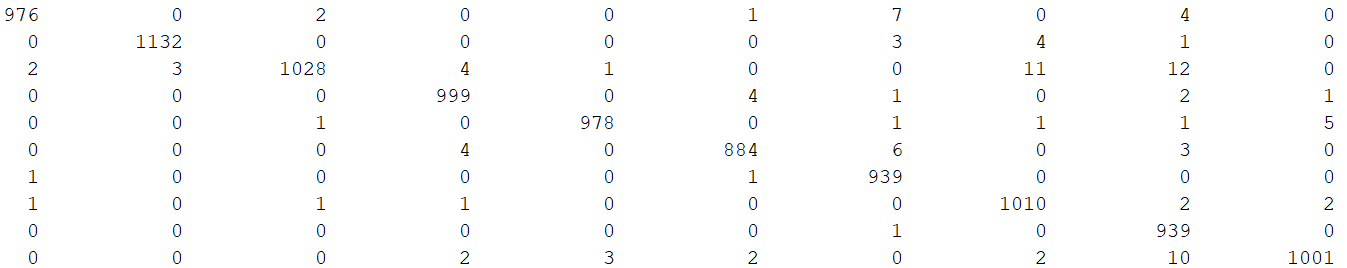
\includegraphics[width=0.95\textwidth]{cnn_confusion_matrix.png}}}
			\caption{CNN Confusion Matrix}
			\label{cnn_confusion_matrix}
		\end{figure}
		
		When evaluated on the test data set, the KNN classifier achieved 94.46\% accuracy. The KNN classification results are displayed in the following confusion matrix:
		
		\begin{figure}[H]
			\centerline{\fbox{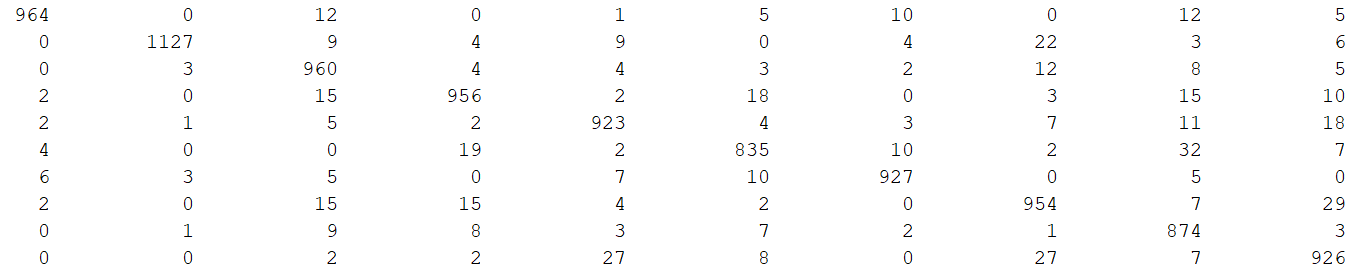
\includegraphics[width=0.95\textwidth]{knn_confusion_matrix.png}}}
			\caption{KNN Confusion Matrix for K=3}
			\label{knn_confusion_matrix}
		\end{figure}		
	
		The CNN classifier achieved better performance than the KNN classifier. It not only achieved a higher overall accuracy, but it also provided better performance for samples of all input classes. (This can be seen on the main diagonal of the confusion matrix.)
	
	\end{enumerate}
	
	\pagebreak
	\appendix
	\section{CNN Code}
	\label{cnn_code}
	\lstset{style=Matlab-editor,basicstyle=\ttfamily\footnotesize}
	\lstinputlisting{Homework5_Sowatzke.m}
	\lstinputlisting{loadMNISTData.m}
	\lstinputlisting{readBinaryFile.m}
	\raggedbottom
\end{document}